%%%%%%%%%%%%%%%%%%%%%%% file template.tex %%%%%%%%%%%%%%%%%%%%%%%%%
%
% This is a general template file for the LaTeX package SVJour3
% for Springer journals.          Springer Heidelberg 2010/09/16
%
% Copy it to a new file with a new name and use it as the basis
% for your article. Delete % signs as needed.
%
% This template includes a few options for different layouts and
% content for various journals. Please consult a previous issue of
% your journal as needed.
%
%%%%%%%%%%%%%%%%%%%%%%%%%%%%%%%%%%%%%%%%%%%%%%%%%%%%%%%%%%%%%%%%%%%
%
% First comes an example EPS file -- just ignore it and
% proceed on the \documentclass line
% your LaTeX will extract the file if required






\begin{filecontents*}{example.eps}
%!PS-Adobe-3.0 EPSF-3.0
%%BoundingBox: 19 19 221 221
%%CreationDate: Mon Sep 29 1997
%%Creator: programmed by hand (JK)
%%EndComments
gsave
newpath
  20 20 moveto
  20 220 lineto
  220 220 lineto
  220 20 lineto
closepath
2 setlinewidth
gsave
  .4 setgray fill
grestore
stroke
grestore
\end{filecontents*}
%
\RequirePackage{fix-cm}
%
%\documentclass{svjour3}                     % onecolumn (standard format)
%\documentclass[smallcondensed]{svjour3}     % onecolumn (ditto)
%\documentclass[smallextended]{svjour3}       % onecolumn (second format)
\documentclass[twocolumn]{svjour3}          % twocolumn
%
\smartqed  % flush right qed marks, e.g. at end of proof
%
\usepackage{graphicx}

\usepackage{amsmath} 
\usepackage{amssymb}

\usepackage{multirow}
\usepackage{float}
\restylefloat{table}

\newtheorem{thm}{Theorem}



%
% \usepackage{mathptmx}      % use Times fonts if available on your TeX system
%
% insert here the call for the packages your document requires
%\usepackage{latexsym}
% etc.
%
% please place your own definitions here and don't use \def but
% \newcommand{}{}
%
% Insert the name of "your journal" with
% \journalname{myjournal}
%
\begin{document}

\title{Computing the Log Concave NPMLE for Interval Censored Data%\thanks{Grants or other notes
%about the article that should go on the front page should be
%placed here. General acknowledgments should be placed at the end of the article.}
}
%\subtitle{Do you have a subtitle?\\ If so, write it here}

%\titlerunning{Short form of title}        % if too long for running head

\author{Clifford Anderson-Bergman         \and
        Yaming Yu %etc.
}

%\authorrunning{Short form of author list} % if too long for running head

\institute{Clifford Anderson-Bergman \at
              367 Evans Hall, Department of Statistics, UC Berkeley, Berkeley, CA 94720  \\
              Tel.: 415-350-3209\\
%              Fax: +123-45-678910\\
              \email{cianders@berkeley.edu}           %  \\
%             \emph{Present address:} of F. Author  %  if needed
           \and
           Yaming Yu \at
              Department of Statistics, UC Irvine, Irvine, CA 92697 
}

\date{Received: date / Accepted: date}
% The correct dates will be entered by the editor


\maketitle

\begin{abstract}

	In analyzing interval censored data, a non-parametric estimator is often desired due to difficulties in assessing model fits. Because of this, the non-parametric maximum likelihood estimator (NPMLE) is often the default estimator. However, the estimates for values of interest of the survival function, such as the quantiles, have very large standard errors due to the jagged form of the estimator. By forcing the estimator to be constrained to the class of log concave functions, the estimator is ensured to have a smooth survival estimate which has much better operating characteristics than the unconstrained NPMLE, without needing to specify a parametric family or smoothing parameter. In this paper, we first prove that the likelihood can be maximized under a finite set of parameters under mild conditions, although the log likelihood function is not strictly concave. We then present an efficient algorithm for computing a local maximum of the likelihood function. Using our fast new algorithm, we present evidence from simulated current status data suggesting that the rate of convergence of the log-concave estimator is faster (between $n^{2/5}$ and $n^{1/2}$) than the unconstrained NPMLE (between $n^{1/3}$ and $n^{1/2}$).
\\
\keywords{Interval Censored Data \and Shape Constraints \and Log-Concave \and NPMLE}
% \PACS{PACS code1 \and PACS code2 \and more}
% \subclass{MSC code1 \and MSC code2 \and more}
\end{abstract}

{\section{Introduction}
\label{sec:intro}	}

	The NPMLE is a popular estimator for interval censored data \cite{RefT1976}, the main strength being the flexibility of the model. A flexible estimator is especially important for interval censored data, as assessing model fit can be difficult. However, this comes at the cost of high variability of survival estimates. In particular, the convergence rate of the NPMLE has been shown to be $n^{1/3}$ for current status data \cite{RefG1987}. For case II interval censored data, the convergence rate is more complicated, being shown to be between $ n^{1/3}$ \cite{RefG1991} and $n^{1/2}$ \cite{RefH1999} depending on the severity of the censoring. Heuristically, the poor behavior of the NPMLE is due to the fact that the estimated survival curves are similar to step functions with a relatively small number of steps, even for larger datasets.

	Parametric models allow for much more efficient estimation, providing $n^{1/2}$ convergence rates. This depends on parametric assumptions which are hard to assess for interval censored data and can lead to heavy bias in survival estimates if inappropriate. Because of this, parametric models are fairly unpopular for use in interval censored data. 	
	
	Alternatively, issues of the erratic nature of the NPMLE can be remedied by making an assumption about the smoothness of the underlying distribution, rather than making an assumption of belonging to a parametric family.  This is often done by introducing a smoothness parameter. One method for smoothing with interval censored data is the kernel density estimator \cite{RefBea2005}, which requires selection of a bandwidth parameter. Another technique is the log-spline density estimator, using a smoothness penalty to select the number of knots \cite{RefKS1992}. While both of these techniques have been shown to reduce the variance of the estimated survival curve for interval censored data \cite{RefP2000}, they have their drawbacks. Both these estimators require selecting an nonintuitive smoothness parameter. At this moment, neither method has a well justified smoothness selection rule that we are aware of. While both these methods may prove fruitful if automated smoothness parameter selection methods can be developed specifically for interval censored data, in our study we found current implementations of such rules unreliable (implementations are available in CRAN \cite{R} packages ICE \cite{R_ICE} and logspline \cite{R_logSpline}). This produces demand for a fully automated, theoretically justified smooth estimator. 
	
	%(CRAN packages \texttt{ICE} and \texttt{logspline} use ad-hoc methods that can lead serious estimation problems with heavily censored data). 
	
	%As an example, the logspline density estimator can be found in the CRAN package  ``logspline", with preset smoothing penalties. While this estimator can perform well with light censoring, in our experience with simulated data it behaved poorly under heavy censoring. In particular, it was often observed that either the algorithm fails to converge when used with current status data, even for large data sets (in fact, the estimator appears to perform \emph{worse} for larger data sets). Similar problems were noted in \cite{RefP2000}.  Likewise, the question of bandwidth selection for the kernel smoother in application to interval censored data is still an open question. Currently the CRAN kernel smoothing for interval censored data package ``ICE" uses the ad-hoc method of imputing the censored data and using standard uncensored methods for selection of bandwidth. We found that this can lead to heavy bias of the survival estimates in many cases with simulated data.  
	 
	
		
	Another approach is to apply a flexible shape constraint which results in a smooth survival function \cite{RefDFJ2006}, \cite{RefDea2014}. We focus on the popular shape constraint of log concavity \cite{RefBB2005}. A density function $f_X(x)$ is considered log-concave if $f_X(x) = e^{\varphi(x)}$, where $\varphi$ is a concave function. This will ensure that $f_X(x)$ will not have more than one peak (but can be flat, such as a uniform distribution). Because a straight line is on the boundary of log-concave functions, it ensures the tails of the distribution are at most exponential (\emph{i.e.} log-linear). This assumption is considered very flexible as many parametric distributions fit into this category. The families of log-concave distributions include normal, gamma with shape parameter $\ge$ 1, all Weibull densities with exponent $\ge$ 1, all beta densities with both parameters $\ge$ 1 and the logistic density. Non-logconcave distributions include the t-distribution, the lognormal distribution and any multimodal distribution. This estimator is a consistent estimator of the density in the case of exact data \cite{RefDR2009} and an efficient algorithm for finding the log-concave NPMLE has been written for uncensored data \cite{RefDea2007}. 

	An outline for an EM algorithm for finding the log-concave NPMLE (also paired with a cure rate parameter) for interval censored data first appeared in \cite{RefDea2007}. This algorithm was formally published, along with proof of consistency of the estimator for interval censored data, in \cite{RefDea2014}. The algorithm which was presented discretizes the domain and applies an EM algorithm to find an approximation of the log-concave NPMLE with the option of including a cure rate parameter (only an approximation due to the discretizing of the data). This algorithm has been implemented in the CRAN package logconcens \cite{R_logconcens}. In practice we found this algorithm to be too slow for moderately sized data sets with interval censored data. While a more efficient implementation would likely speed up computation (logconcens uses both R and C++ for computation), it seems unlikely that this EM algorithm will be able to handle larger datasets quickly. The EM algorithm uses the same missing data scheme as in Turnbull's EM algorithm \cite{RefT1976} for computing the unconstrained NPMLE for interval censored data. This algorithm is known to be quite slow for the unconstrained NPMLE \cite{RefJ1998}, in which the M step is in closed form, unlike the log-concave NPMLE which must use sequential quadratic programming for the M step. In fact, we found that this algorithm occasionally failed to converge after 1,000 iterations (between 0\% and 17\% across the different simulated datasets we considered) and would still be fairly far away from the local maximum it was approaching after these 1,000 iterations. In addition to slow convergence in iterations, the discretization increases the dimensions of the parameter space significantly, requiring more time per iteration. This leads to demand for a fast and reliable algorithm for finding the log-concave NPMLE for interval censored data. 
	
	
	%We found this algorithm frequently failed to converge after 1,000 iterations (between 15\% and 67\% in the different sizes of datasets we concerned) and would still be fairly far away from the local maximum it was approaching after these 1,000 iterations. Default settings on the package set the maximum iterations to 49. Even when the algorithm did converge, it was found to be too slow for most purposes (see table \ref{table:LogConSpd} for average speeds and frequency of failure to converge). This result is not surprising, given that the algorithm used in logconcens is very similar in structure to the standard EM algorithm for the unconstrained NPMLE \cite{RefT1976}. This algorithm is notoriously slow even for the unconstrained NPMLE \cite{RefJ1998}, in which the M step is in closed form, unlike the log-concave NPMLE which must use sequential quadratic programming for the M step. This leads to demand for an fast and reliable algorithm for finding the log-concave NPMLE for interval censored data. 
		
	In this paper, we first provide a theorem which shows that the log-concave NPMLE can be characterized using a finite number of parameters (note: a very similar theorem can be found in \cite{RefDea2014} and was originally published in \cite{myThesis}). Using this theorem, rather than discretizing the data, we construct an efficient method for finding a local maximum of the likelihood function. Although the log likelihood function is not strictly  concave, starting from random starting values resulted in similar final estimates, suggesting multi-modality is not likely to be a significant problem. Unlike the algorithm found in logconcens, this algorithm almost never failed to converge after 1,000 iterations ($< 0.1\%$ in the settings we considered) and was typically hundreds to thousands of times faster than the algorithm found in logconcens. In the illustrative example used in this paper ($n = 4,386$), our algorithm found the log concave NPMLE in 0.584 seconds (final log likelihood = -5560.940). In contrast, the algorithm found in logconcens took 1,613 seconds (final log likelihood = -5560.945). With our new algorithm, we examined the empirical rate of convergence of survival estimates and compare to those of the unconstrained NPMLE. 
	
	The organization of the rest of this paper is as follows.  In section \ref{sec:llk}, we formulate the likelihood function that we are interested in maximizing. In section \ref{sec:s_set}, we prove a theorem which shows that the likelihood achieved from any log concave density function is less than or equal to the likelihood which can be achieved by a log linear spline with a finite number of knots. With this finite parameterization, we show that the maximum likelihood exists under minimal conditions. In section \ref{sec:params}, we present the different parameterizations that will be used in the algorithm. In section \ref{sec:asa}, we describe the algorithm itself. In section \ref{sec:ME}, we apply the algorithm to a classic data set. In section \ref{sec:AlgSpd}, we compare the speed of our algorithm with the algorithm found in logconcens. In section \ref{sec:Conv}, we compare the rate of convergence of the log-concave NPLME with the unconstrained NPMLE via simulation. In section \ref{sec:future}, we discuss future research topics for the log-concave NPMLE. In section \ref{sec:software}, we present the CRAN package where this algorithm can be found. 
\\

{\section{Likelihood Function}
\label{sec:llk}}

	We consider the univariate survival scenario and adopt the standard assumption of independent observations among subjects and an independent censoring mechanism. For the $i^{\mathrm{th} } $ subject, suppose the exact event time is known to be within the observation interval $[L_i, R_i]$.  Note that this allows for right censoring ($R_i = \infty$, although this is a slight abuse of notation), left censoring ($L_i = 0$) or uncensored data points ($L_i = R_i$). Let $\phi(x)$ represent the log density at time $x$. Because we are dealing with proper density estimates (unlike the unconstrained NPMLE), we must use the standard survival notation of $\delta_i = I_{ \{ L_i = R_i \} }$ (\emph{i.e.}\ $\delta_i$ is an indicator that subject $i$ was uncensored).  Then the log likelihood function is 
	
	\[\ell(\phi) = \displaystyle \sum_{i = 1}^n \delta_i \phi(L_i)   + (1 - \delta_i) \log \left[ S(R_i) - S(L_i) \right]
	\]
	
	where 
	\[
	S(R_i)  - S(L_i) = \int_{L_i}^{R_i} e^ { \phi(x) } \,\mathrm{d}x  
	\]
	
	From this, the log-concave NPMLE is 
	
	\[ \hat \phi = \underset{\phi} {\arg \max}   \displaystyle \sum_{i = 1}^n \delta_i \phi(L_i)   + (1 - \delta_i) \log \left[ S(R_i) - S(L_i) \right] 
	\]
	which satisfies 
	\[
	 \quad \frac{ \phi(x_2) - \phi(x_1)} {x_2 - x_1} \geq \frac{ \phi(x_3) - \phi(x_2)} {x_3 - x_2} \quad \forall x_1 < x_2 < x_3 
	 \]
	 where $\phi(x)$ is defined and 
	 \[ 
	 \int_{-\infty}^{\infty} e^{\phi (x) } \mathrm{d}x = 1
	\]

	To ease the last restriction, we replace $e^{\phi(x)}$ with $\frac{e^{\phi(x)} } { \int_{-\infty}^{\infty}  e^{\phi(x)} \mathrm{d}x}$, so that $e^{\hat \phi(x)}$ is proportional to the log-concave NPMLE. Under this parameterization, the log-concave NPMLE is written as 

	\[ \hat \phi ={\phi}_{\arg \max} \displaystyle \sum_{i = 1}^n \delta_i \phi(L_i)   + (1 - \delta_i) \log \left( \int_{L_i}^{R_i} e^ { \phi(x) } \,\mathrm{d}x \right) \]
	\[
	- n \times \log \left(  \int_{-\infty}^{\infty} e^ { \phi(x) } \mathrm{d}x \right) 
	\]
	which satisfies
	\[
	 \quad \frac{ \phi(x_2) - \phi(x_1)} {x_2 - x_1} \geq \frac{ \phi(x_3) - \phi(x_2)} {x_3 - x_2}\quad \forall x_1 < x_2 < x_3 
	 \]
	
	Note that under this parameterization, $\hat \phi(x)$ is calculated up to an additive constant. For simplicity we set $\max_x $ $\hat \phi(x) = 0$. We can then interpret $\hat \phi(x)$ as the estimated log ratio between the density at $x$ and the density at the mode.
\\

{ \section{Solution Set}
\label{sec:s_set} }

In the case of only uncensored observations, it is known that the log concave NPMLE must be a log linear spline, with knots at the observed times and zero density outside the minimum and maximum observed times \cite{RefRuf2007}. To revisit this proof, consider that for exact times the log likelihood function can be written as	
	\[ \displaystyle \sum_{i = 1}^n \phi(x_i) - n \times \log \int e^{\phi(x)} dx
	\]
where $x_1<x_2<\cdots<x_n$ are the ordered observations. For a fixed set of values of $\phi(x_i)$, the likelihood is maximized by minimizing $\int e^{\phi(x)} dx$. For fixed $\phi(x_i)$ and $\phi(x_{i+1})$, $\int_{x_i}^{x_{i+1}} e^{\phi(x)}dx$ under the concave restriction of $\phi(x)$ is minimized by linearly connecting $\phi(x_i)$ and $\phi(x_{i+1})$. Thus, $\hat \phi(x)$ is a log linear spline with knots at the observed times in the case of exact observations. The concavity of the log-likelihood function with exact observations ensures that the solution exists and is unique.
		
	In the case of interval censored data, the LC NPMLE is not necessarily unique. As a trivial example, consider the case $n = 1$. In such a case, any log concave function which places all of the mass inside of the observed interval would be an LC NPMLE. This is very similar to the problem of representational non-uniqueness in the unconstrained case \cite{RefGV2002}. With such issues in mind, we instead first show that the log likelihood achieved by any log-concave function can be matched by the log likelihood from a log linear spline with a finite number of knots, while recognizing that there may be other functions which have the same likelihood. After this, we use this finite parametrization to prove that the maximum likelihood exists under minimal conditions. 
	

	\vspace{3mm}

	\begin{thm}
	\label{thm1}
	Define $u_t$ = number of unique values of $L_i$ and $R_i$. If the maximum likelihood exists, it can be can be achieved with a log linear spline with at most $2u_t-1$ knots.
	\end{thm}
	
\begin{figure}[h]
\centerline{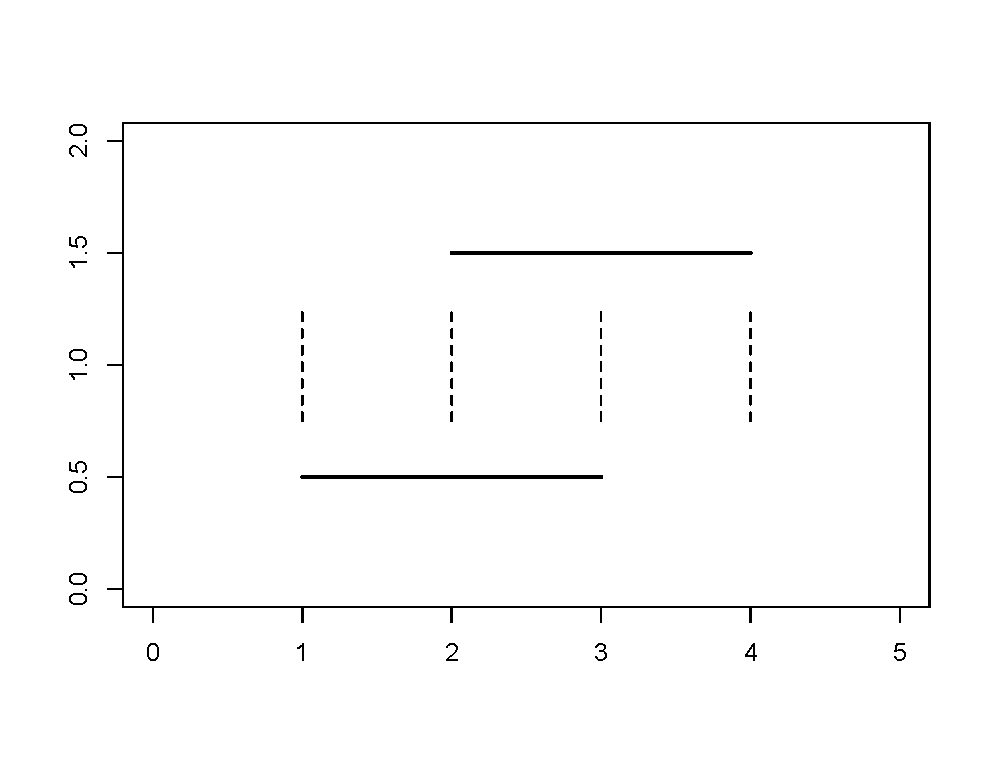
\includegraphics[width = 8cm]{ContrbInt.pdf} }
\caption{Observation intervals and contribution intervals}
\label{figure:ObsInt}
\end{figure}	

	\begin{proof}

	Define the $i^{\text{th}}$ observation interval $[L_i, R_i]$ to be the interval in which the $i^{\text{th}}$ event was known to have occurred (note: we allow for $L_i = R_i$, or an interval of length 0). Define a contribution interval to be an interval such that both ends of the interval are ends of (potentially different) observation intervals, with no other ends of observation intervals in between. For example, Figure \ref{figure:ObsInt} shows two observation intervals, $L_1 = 1$, $R_1 = 3$ and $L_2 = 2$, $R_2 = 4$. This leads to 3 contribution intervals; [1,2], [2,3] and [3,4]. Note that exchanging mass \emph{between} contribution intervals will affect the likelihood function, but exchanging mass \emph{within} will not. Also, in any area that is not in a contribution interval, $\phi(x)$ needs to be minimized in the LC NPMLE. Thus, $\hat \phi(x)$ will be linear in areas that are between contribution intervals but are not contribution intervals and $\hat \phi(x)$ will be $-\infty$ in areas that are not contribution intervals and not between contribution intervals. 

	For the $i^{\text{th}}$ contribution interval, define $l_i$ and $r_i$ to be the end points. For given $\phi(l_i)$, $\phi'(l_i -)$ (left derivative at $l_i$), $\phi(r_i)$ and $\phi'(r_i+)$ (right derivative at $r_i$), this contribution interval affects the likelihood only through the total mass assigned to it, $i.e.$ $p_i = \int_{l_i}^{r_i} e^ {\phi(x)} dx$ (note: under this parameterization, it is not necessary that $\sum p_i = 1$). Note that $p_i$ is minimized by making $\phi(x)$ linear on $(l_i, r_i)$. If $\phi'(l_i - )$ = $\phi'(r_i + )$, then by concavity $\hat{\phi}(x)$ must be linear over $(l_i, r_i)$ and no knots are needed in the interval. If not, we will need to add another knot. Let us define a point $m_i$ inside the contribution interval to be the horizontal coordinate of the intersection of the two lines

	\[
	y_1 = \phi(l_i) + (x - l_i) \phi'(l_i-)
	\]	
	
	and 
	
	\[
	y_2 = \phi(r_i) + (x - r_i) \phi'(r_i+)
	\]
	
	which are the linear extensions of $\phi(x)$ on $(l_i, r_i)$ (note: we owe this simple description of $m_i$ to one of our anonymous reviewers, which is much easier to follow than our original explanation).  It is worth recalling that because $\phi$ must be a concave function, in general $\phi'(l_i) \ge \phi'(r_i)$, and in this case that we are considering $\phi'(l_i) > \phi'(r_i)$, implying $l_i < m_i < r_i$. Solving for $m_i$, we get 
	 	
	\[ m_i = \frac{\phi(r_i) - \phi'(r_i + ) r_i - \phi(l_i) + \phi'(l_i - ) l_i} { \phi'(l_i - ) - \phi'(r_i + )}.
	\]		
	 We can maximize $p_i$ by setting $\phi(m_i)$ to the vertical value of this intersection, as seen in Figure \ref{figure:MaxMin}. 

	\begin{figure}[h]
\centerline{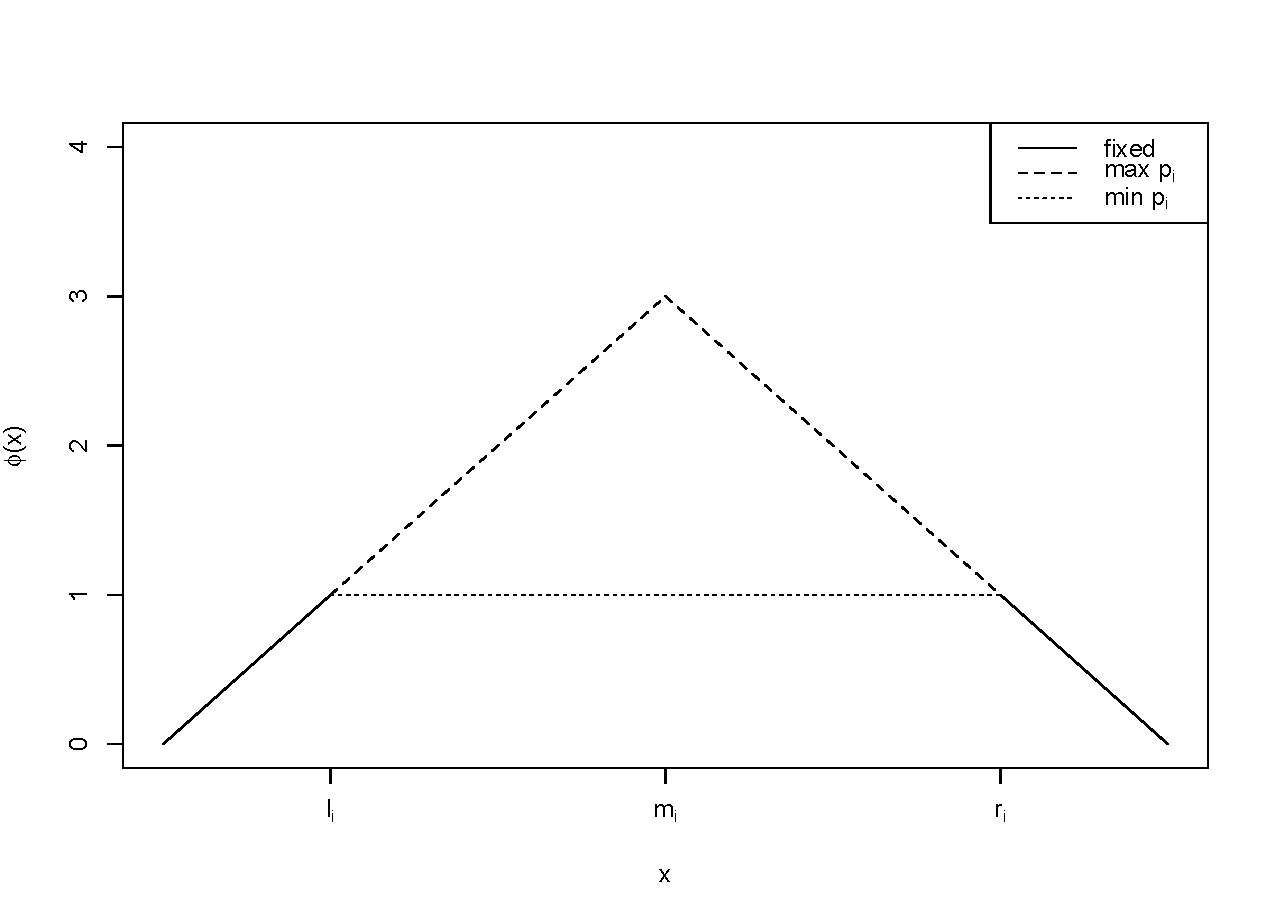
\includegraphics[width = 9cm]{maxminpk.pdf}}
\caption{Maximizing and Minimizing $p_i$}
\label{figure:MaxMin}
\end{figure}		

	Therefore, by adding a knot at $m_i$, we can set $p_i$ to either the minimum or the maximum possible under the log concavity constraint, with given $\phi(l_i)$, $\phi'(l_i -)$, $\phi(r_i)$ and $\phi'(r_i+)$. In fact, we can set $p_i$ to any value between the minimum and maximum by setting $\phi(m_i)$ to a suitable value between its minimum and maximum allowed by the constraints.  In other words, whatever likelihood value can be achieved by an arbitrary log-concave density, we can also achieve by a log linear spline with knots at the end points of contribution intervals and (if needed) one knot inside each contribution interval. This leads to a maximum of $2u_t-1$ necessary knots.
	
	Two special cases to consider are if an observation is uncensored and if a contribution interval is unbounded on the right. If an observation is uncensored, this results in a contribution interval that is of length 0, and so $l_i$, $r_i$ and $m_i$ are equivalent and only a single knot will be needed. Other than that, the same rules will apply in the same fashion. For example, if we have observation interval [1, 3] and an uncensored observation at 2, then the contribution intervals would be [1,2], [2,2] and [2,3]. We then need knots at 1, 2 and 3 and knots inside [1,2] and [2,3]. In the case of a contribution interval in which $r_i = \infty$, we note that $m_i$ will be undefined. However, in this case, by allowing the slope to change inside the contribution interval, without adding any knots, we can allow the probability mass to span all values between the min and max mass assigned. In practice, we implemented this by setting $m_i = l_i + 1$ and enforcing that $\phi'(m_i+) = \phi'(l_i+)$. While this required us to handle the final knots as special cases when evaluating the log likelihood function, it meant that we could treat the constraint of log concavity in the same fashion for all knots, rather than including a slope parameter at the ends. If negative event times are allowed, a similar strategy would be used for $l_i = -\infty$. 
	
	\end{proof}
	
	Theorem~\ref{thm1} is important as it clarifies the form of the NPMLE.  However, without knowing $\hat\phi(x)$, one cannot know the exact location of $m_i$ for the $i^{\text{th}}$ contribution interval. In order to deal with this, $m_i$ is replaced with the fixed location $mid_i = \frac{l_i + r_i}{2}$ for the main portion of the algorithm, as $mid_i$ should be close to $m_i$. Once the solution is sufficiently close, we allow the midpoints to move and consider $m_i$ as another set of parameters we must optimize over. This will be discussed in section 6.3. 
		
	Using this parameterization, we can prove that the likelihood function has a maximum under the following mild condition. 
		
	\begin{thm}
	\label{thm2}
	The likelihood function is continuous, coercive and bounded (and therefore has a maximum) if there exists $i,j \in 1, ... , n$ such that $L_i > R_j$. 
	
%	at least one of the following three conditions is met:
	
%	1. All the data are censored and at least two of the observations do not overlap
	
%	2. At least two data points are uncensored, and they are not equal to each other
	
%	3. There exists one uncensored data point which is not contained in at least one of the censored intervals
	
	
	\end{thm}
	
	See appendix for a proof of this theorem. 	
	\\
	{\section{Parameterizations} 
	\label{sec:params}	}

	The algorithm presented in this paper uses an active set algorithm, very similar to the algorithm used in the case of uncensored times \cite{RefRuf2007}. In order to clearly define the active set algorithm, several definitions are required. To start with, we define $\beta_i = \phi(x_i)$, where $x_i$ is the location of the $i^{\text{th}}$ knot as described in Theorem \ref{thm1}. Let $k$ be the total number of knots. Because $\phi(x)$ is a linear spline with knots at the $x_i$'s, the values of $\beta_1, \beta_2, ..., \beta_k$ and $x_1, x_2,..., x_k$ will completely characterize $\phi(x)$. This will be referred to as the simple parameterization. We also denote $\Delta_i = \frac{\beta_{i+1} - \beta_i} {x_{i+1} - x_i}$. With this notation, we note that the constraint of log concavity is equivalent to $\Delta_1 \geq \Delta_2 \geq ... \geq \Delta_{k-1}$. In principal, we would like to define $x_i$ to be active if $\Delta_{i-1} > \Delta_i$ and inactive if $\Delta_{i-1} = \Delta_i$. However, due to numerical errors in calculating $\Delta_i$, we define $x_i$ to be active if $\Delta_{i-1} > \Delta_i + \xi$ and inactive if $\Delta_{i-1} \leq \Delta_i + \xi$.  We set $\xi = 10^{-13}$ and found no problems resulting from this. 
	
	Similar to the case of exact times \cite{RefRuf2007}, we noticed that the solution tends to have very few active points compared to total number of points considered. We can take advantage of this to create an efficient algorithm using an active set parameterization. Under this parameterization, we treat $\phi(x)$ as a linear spline with knots only at the active points, instead of all the points. We use the notation $\beta_i^*$ to denote the active set parameterization. The values of the parameters remain the same,  ($\beta_i^* = \beta_i$), but when we increase $\beta_i^*$, we also increase the neighboring inactive $\beta_j$ as though the only knots were at the active points, i.e. the inactive $\beta_j$ are determined by linear interpolation from the nearest active points. To illustrate this, figure 4 demonstrates adding 1 to $\beta_4^*$, which takes an inactive point and makes it active under the active set parameterization. To formally characterize addition under the active set parameterization, define $a(m)$ to be the index of the $m^{\text{th}}$ active point. If $i = a(m)$ then $\beta_i^{*(t+1)} = \beta_i^{*(t)} + h$ is equivalent to 
		
	\[
	\beta^{(t+1)}_j = 
	\begin{cases}
		\beta^{(t)}_j + h \times \frac{x_j - x_{a(m-1)} } {x_{i} - x_{a(m-1)} } , &  \textrm{if } x_{a(m-1)} < x_j  \leq x_{i} \\  
		\beta^{(t)}_j + h \times \frac{x_{a(m+1)} - x_j} {x_{a(m+1)} - x_{i} }, & \textrm{if } x_{ i} < x_j < x_{a(m+1)} \\ 
		\beta^{(t)}_j,  \textrm{otherwise}
	\end{cases}
	\]

	
\begin{figure}[h]
\centerline{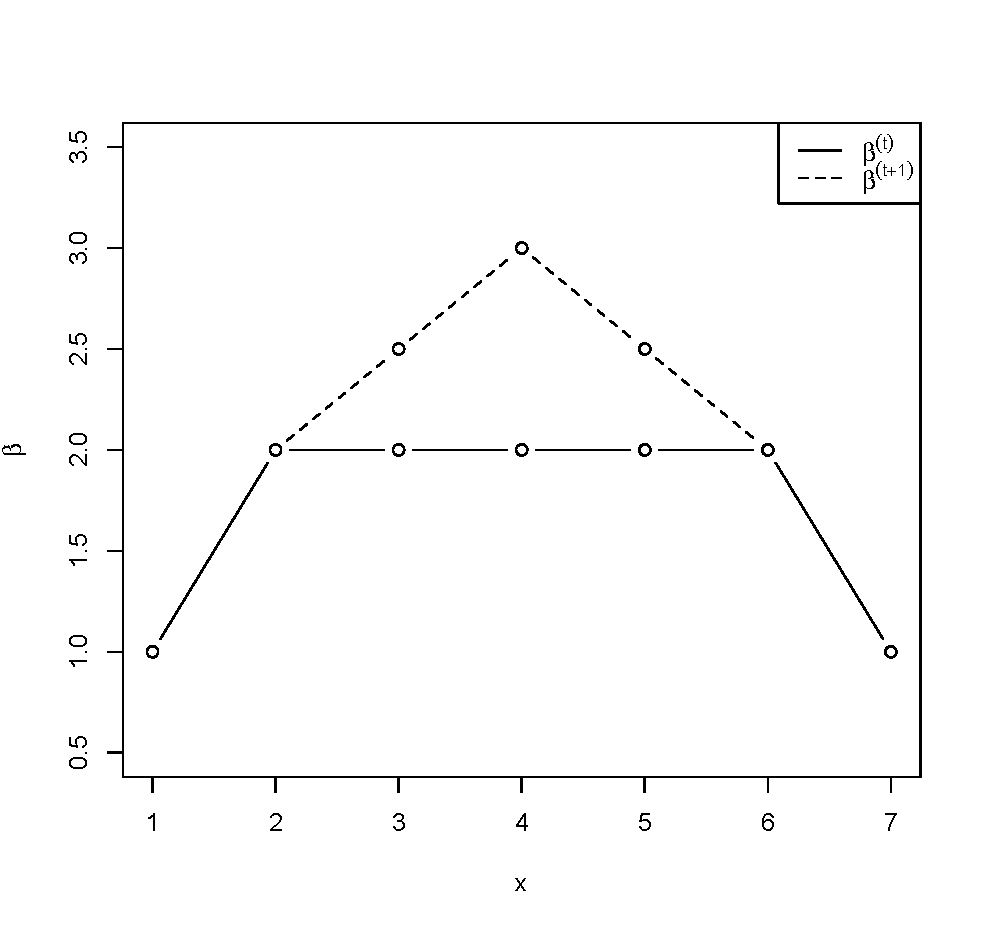
\includegraphics[width = 8cm]{ActivePoint.pdf}}
\caption{$\beta_4^{*(t+1)} = \beta_4^{*(t) }+1$}
\label{figure:ActPt}
\end{figure}		
		
	Under the active set parameterization, all active points have a neighborhood for which they can both increase and decrease without violating the condition of logconcavity. Inactive points have a neighborhood in which they can increase and become an active point, but cannot decrease. In contrast, under the simple parameterization, inactive points cannot decrease and all points can increase only if the neighboring points are active. For example, in figure \ref{figure:ActPt}, $\beta_4^{(t + 1)} = \beta_4^{(t)} + 1$ (\emph{i.e.} using the simple parameterization) violates log concavity, but $\beta_4^{*(t+1)} = \beta_4^{*(t)} + 1$ (\emph{i.e.} using the active set parameterization) does not. 
	
	In a slight abuse of notation, let us also define $\Delta_{a(i)} = \frac{\beta_{a(i + 1)} - \beta_{a(i)} } {x_{a(i + 1)} - x_{a(i)} }$. If $K$ = number of active points, then $\Delta_1 \geq \Delta_2 \geq ... \geq \Delta_{k-1}$ is equivalent to $\Delta_{a(1)} \geq \Delta_{a(2)} \geq ... \geq \Delta_{a(K-1)}$ (up to numeric error). 

	In choosing which active set parameter to optimize, we will use what we call the KKT error, based on the KKT conditions \cite{RefKKT1951}. Let us define
	
	\[
	\textrm{KKT error} = {\textrm{max}} 
	\begin{cases}
		|\frac{\partial \ell } {\partial \beta_i^*}|,  \textrm{if } \Delta_{i-1} > \Delta_{i} + \xi \\
		\textrm{max}(\frac{\partial \ell}{\partial \beta_i^*},0 ) ,  \textrm{if } \Delta_{i-1} \leq \Delta_i + \xi \\  
	\end{cases}
	\]
	
	In other words, the KKT error is the maximum of the absolute value of the derivatives associated with the active set parameterization of all the active points and the positive derivatives associated with the active set parameterization of the inactive points (because decreasing would violate the log concavity restraint). This will be used in a step in our algorithm to chose which parameter to update. 
\\



{\section{Active Set Algorithm} 
\label{sec:asa}	}

	Each iteration of the algorithm includes four steps: one which selects new points to add to the set of active points (similar to the VDM algorithm \cite{RefF1972}), one which efficiently increases the likelihood over the set of currently active points (similar to the methods used to compute the log-concave NPMLE with uncensored observations \cite{RefDea2014}), one that fixes the tails and one that moves the location of the active points. The first step selects the index $i$ with the maximal error and uses simple univariate techniques to find an optimal $\beta_i^*$. The second step optimizes over the active set by approximating the log-likelihood function with a second order Taylor expansion, and then maximizing this approximation using quadratic programming, similar to the ICM algorithm \cite{RefJ1998}.  Because often $\beta_i = -\infty$ on the tails at the solution, it is occasionally necessary to adjust the tails of $\beta$ for numerical stability which is done in the fixing tails step. Finally, after the solution is sufficiently close (\emph{i.e.} maximum change in all parameter values is less than $\epsilon_m$), we allow the location of the active points to move via Newton's method. The algorithm is terminated when the maximum change in all parameter values is less than $\epsilon_t$. In our algorithm, we chose to set $\epsilon_m = 10^{-2}$ and $\epsilon_t = 10^{-5}$. 
	
	 The basic form of the algorithm is as follows:
	
	\vspace{3mm}
	
	\begin{itemize}
	
		\item Set initial values for $\beta$ 
		
		\item Set MOVEX = FALSE
		
		\item Set $err$ = $\infty$

		
		\item While ($err > \epsilon_t$ and $t <$ max iterations)
		
		\{
		
			\begin{itemize}
			
			\item $t = t + 1$
										
			\item Select index $i$ with maximum KKT error 
			
			\item Use univariate optimization to update $\beta_i^{*(t)}$
						
			\item Use quadratic programming to optimize over active set
			
			\item Fix tails of $\beta^{(t)}$ if necessary
						
			\item $err$ =  max($| \beta_i^{(t)} - \beta_i^{(t-1)}|$) 
			
			\item If($err < \epsilon_m$)
				
				\begin{itemize}
				
				\item MOVEX = TRUE
				
				\end{itemize}
			
			\item If(MOVEX == TRUE)
				
				\{
				
				\begin{itemize}
										
				\item Use bivariate Newton's method to update knot location of active points which are midpoints
				
				\item $err$ =  max($err$, $| x_i^{(t)} - x_i^{(t-1)}|$) 
				
				\end{itemize}
			
				\}
						
			\end{itemize}
			
	\}
	
	\item Convert $\beta$ to $e^{\phi(x)} / \int e ^ {\phi(x)} \mathrm{d}x$
	
	\item Return $e^{\phi(x)} / \int e ^ {\phi(x)}\mathrm{d}x$
	
	\end{itemize}
	
	It is important to note that after the MOVEX part of the algorithm is activated, we still need to update all values of $\beta_i$, as moving the location of the knots will cause a change in the constraints. 
	
	There is one technical note about the initial values of $\beta$. It is very tempting to start with a uniform set, \emph{i.e.} $\beta_1 = ... = \beta_k = 0$. However, if the censoring is over an infinite area ($R_i = \infty$ or $L_i = -\infty$), this will result in an improper distribution, as the distribution Uniform$(a, \infty)$ is improper. To ensure the initial distribution is properly defined, we set $m$ = $\frac{k + 1} {2}$ and set $\beta_i = -|x_m - x_i | / \sigma_x^*$, where $\sigma_x^*$ is the standard deviation of all finite locations of the knots. This leads to a Laplace distribution if defined on $\mathbb{R}$ and a truncated Laplace distribution otherwise.	
	\\
	
	{\subsection{Univariate Optimization}} 
	
	Our algorithm selects the index $i$ associated with the maximum KKT error. Once the index $i$ is selected, $\beta_i^*$ must be selected which increases the likelihood. Let $i = a(j)$ (if $i$ is not an active point, it will be after optimization). From the constraints $\Delta_{a(j-2)} \geq \Delta_{a(j-1)}$, $\Delta_{a(j-1)} \geq \Delta_{a(j)}$ and $\Delta_{a(j)} \geq \Delta_{a(j+1)}$, we derive the constraints
	
	\[
	 \beta_i^* \leq \text{min} (\beta_{a(j-1)} + \Delta_{a(j-2)} \times (x_{a(j)} - x_{a(j-1)}),
	 \]
	 \[
	 \beta_{a(j+1)} -\Delta_{a(j+1)} \times (x_{a(j+1)} - x_{a(j)}) ) 
	\]
	
	\[
	 \beta_i^* \geq \left(\frac{1}{x_{a(j+1)} - x_{a(j)}} +  \frac{1}{x_{a(j)} - x_{a(j-1)} } \right)^{-1} 
	\]
	\[
	\times \left(\frac{\beta_{a(j+1)} } { x_{a(j+1)} - x_{a(j)}} + \frac{\beta_{a(j-1)}} {x_{a(j)} - x_{a(j-1)} } \right)
	\]
	
	Constraints which involve an undefined index, such as $a(0)$, can be ignored. If $\frac{d^2 \ell} {d (\beta^*_{i})^2 } < 0$, then Newton's method was used, subject to the above constraints. Half stepping was used to ensure monotonic convergence. Rarely it was observed that $\frac{d^2 \ell} {d (\beta^*_{i}) ^2 } \geq 0$, in which case the bisection method was used to update $\beta^*_i$. 
	
	Much like the VDM algorithm, these steps alone ensure that the algorithm will reach a local maximum, but it is observed to do so very slowly. Using simulated data with $n = 200$, we observed that using these steps alone frequently failed to meet the convergence criterion after 1000 iterations, implying that an algorithm based only on univariate optimization would be insufficient. In section 6.3, we present a step that updates all active points simultaneously and greatly accelerates the algorithm. While the multivariate step can be forced to never decrease the likelihood function, the multivariate step alone is not ensured to find a local maximum. Thus, we include both the univariate and multivariate steps in our algorithm to ensure convergence. 
	\\
	
	{\subsection{Maximizing Over an Active Set} }
	
	
	Once given an active set of points, we need a step which can  maximize over the active set efficiently. Because of the linear constraints of concavity, Newton's method is difficult to apply as it would not respect the boundaries. Instead, an ICM \cite{RefJ1998} algorithm is used to maximize over the active set, similar to the algorithm used in the exact case \cite{RefDea2007}. An ICM algorithm works by approximating the target function with a second order Taylor expansion, in which the off diagonal partial derivatives are ignored. In this application, the parameters considered will be the log density at the active points, \emph{i.e.} $\beta_i$'s. It is worth noting that in the traditional ICM algorithm, the off diagonals are ignored due to the expense of computation. In this case the number of parameters considered  is actually fairly low, making the number of off diagonals more manageable, but we have other reasons to ignore the off diagonals which will be discussed shortly. This approximation is maximized, according to the linear constraints, via quadratic programming. We use the notation that a quadratic program minimizes
	
	\[ \frac{1}{2} d^T Q d + c^T d
	\]
	
	Under the constraint \[ A d \leq b\]
	
	We use quadratic programming to minimize the Taylor approximation of $-\ell(\beta^*))$, with the off diagonals of the Hessian ignored. In order to have $\frac{1}{2} d^T Q d + c^T d$ be the given approximation, we define
	
	\[ d_i = \beta^{*(t+1)}_{a(i)} - \beta^{*(t)}_{a(i)}
	\]
	
	\[Q_{i,i} = - \frac{\partial^2 \ell(\beta^{*(t)} )} {\partial {\beta^{*(t)}_{a(i)}}^2}
	\]
	 
	 \[
	 Q_{i,j (i\neq j)} = 0
	 \]
	 
	\[c_i = -\frac{\partial \ell(\beta^{*(t)})} {\partial \beta_{a(i)}^{*(t)} }
	\]
	
	In order to preserve the constraint $\Delta_{a(i)} \geq \Delta_{a(i+1)}$, we set 
	
	\[ A_{i,i} = \frac{1}{x_{a(i+1)} - x_{a(i)} }
	\]
	
	\[ A_{i, i + 1} = \frac{-1}{x_{a(i+1)} - x_{a(i)} } + \frac{-1}{x_{a(i+2)} - x_{a(i + 1)} }
	\]
	
	\[ A_{i, i + 2} = \frac{1}{x_{a(i+2)} - x_{a(i + 1)} }
	\]
	
	\[ b_i =\Delta_{a(i + 1)}^{(t)} - \Delta_{a(i)}^{(t)}
	\]
	
	Similar to the ICM algorithm (Jongbloed 1998), half steps will be taken to ensure the likelihood function does not decrease. In other words, if $\ell ( \beta^{*(t)} + d ) < \ell ( \beta^{*(t)}  ) $, then $d$ is replaced with $d/2$ until $\ell ( \beta^{*(t)} + d ) \geq \ell ( \beta^{*(t)} )$. It was observed that these half steps were required very infrequently. 
	
	Perhaps the most novel part of this algorithm is in how we deal with the fact that $\ell(\beta^*)$ may not be locally concave. In particular, the quadratic function used to approximate the likelihood function will be unbounded if the Hessian is non-negative definite, leading to a degenerate proposed step. Because the ICM algorithm ignores the off diagonals of the Hessian matrix, the only case of concern is when the diagonals of the Hessian are not negative (when the off diagonals are included in the quadratic approximation of the likelihood function, the Hessian was more likely to be non-negative definite). In order to remedy this, an approximation to the second derivative was used which would be ensured to be negative. This approximation takes advantage of the fact that the likelihood function is bounded from above. 
		
	Suppose that the likelihood function is not locally concave as a function of one of the active points, \emph{i.e.}\ $ \frac{\partial^2 \ell} { \partial {(\beta^{*(t)}_{a(i)})}^2} \geq 0$. Let $\tilde \beta^*_{a(i)}$ be the value of $\beta^*_{a(i)}$ that maximizes $\ell(\beta^*_{a(i)})$ in the direction of $ \frac{\partial \ell} {\partial \beta^{*(t)}_{a(i)}} $ (\emph{i.e.}\ if $  \frac{\partial \ell} {\partial \beta^{*(t)}_{a(i)}} > 0$ only consider  $\tilde \beta^*_{a(i)} > \beta^{*(t)}_{a(i)}$, and if $  \frac{\partial \ell} {\partial \beta^{*(t)}_{a(i)}}< 0 $ only consider $\tilde \beta^*_{a(i)} < \beta^{*(t)}_{a(i)}$)  with all other $\beta_{a(j)}$ held fixed. It is worth noting that we don't require $\tilde \beta^*_{a(i)}$ to respect the boundary set by log concavity. If we then consider approximating $\ell(\beta^*_{a(i)})$ with a quadratic function whose first derivative at $\beta^*_{a(i)}$ is $  \frac{\partial \ell} {\partial \beta^{*(t)}_{a(i)}} $ and whose maximum is reached at $\tilde \beta^*_{a(i)}$, this would imply that our approximation of the second derivative would be
	
	 \[\frac{- \left( \frac{\partial \ell} {\partial \beta^{*(t)}_{a(i)} }  \right) } {\tilde \beta^*_{a(i)} -\beta^{*(t)}_{a(i)}}
	 \]
	 
	 This is guaranteed not to be positive.
	
	In the case of a concave likelihood function, half stepping ensures that the likelihood function will increase. Because our target function is not locally concave when using this approximation, even half stepping does not ensure the likelihood function will increase. If after sufficient half steps (we chose 5), the likelihood still does not increase, this step of the algorithm is skipped. Theoretically, if the ICM step repeatedly failed, the algorithm could be extremely slow due to relying only on the univariate optimization. However, this was not observed to occur and substituting this approximation into the ICM algorithm appears to work very well, usually reducing the number of iterations required to below 100 for simulated data of size $n = 200$. While finding  $\tilde \beta^*_{a(i)}$ does come with some computational cost, this approximation was required infrequently and could be done efficiently enough that the computational costs were not significant in the speed of the algorithm. 
	\\
	
		{\subsection{Moving the Knots} } 
	
	Recall that we used $mid_k$ as the location of the knots in the center of each contribution interval because we don't know the exact location defined as $m_k$ in our theorem. To optimize the position of the knots, a bivariate Newton's method was used, with half-stepping of proposed steps to ensure the new proposed estimate increases the likelihood function and respects the constraints. The two parameters considered were the location of the knot (\emph{i.e.}\ $x_i$) and the log density at the knot (\emph{i.e.}\ $\beta_i$). While the log likelihood function does appear consistently to be concave as a function of the location of the knots, we already know that the log likelihood is not always concave as a function of $\beta_i$. In the case where the Hessian matrix is not negative definite, we  perform Newton's method on only the location of the knot and do not update $\beta_i$ in this step (as it will updated in the other steps of the algorithm). The algorithm includes a bisection step for knot location, should the likelihood function be non concave as a function of the knot location, but we have not observed it to be necessary.	We found that it was more computationally efficient to keep the knot locations fixed until the solution was sufficiently close, as dictated by our $\epsilon_m$ trigger. 
		\\
		{\subsection{Fixing the Tails} }
	
	When computing the log-concave NPMLE with exact observations, the area which must have positive mass is known in advance (\emph{i.e.}\ the range of all observed times). When computing the log-concave NPMLE for interval censored data, this not the case, as there are often contribution intervals which receive 0 mass at the log-concave NPMLE. A trivial example to consider is if the data consisted of two overlapping intervals. The log-concave NPMLE would place all the mass in the overlap and no mass to the other two surrounding contribution intervals.% In the case of the unconstrained NPMLE, the mass is known to be positive only in the set of Turnbull intervals. However, the log-concave constraint implies that this is not the case and often some of the contribution intervals outside of the minimum and maximum Turnbull intervals will receive positive mass at the log-concave NPMLE, while others will not.
	 		
	Because of this, simply allowing the earlier steps to find the log densities	 at the tails of the estimated density can lead to numerical instability as $\beta_i \rightarrow -\infty$. Numerical instability typically happened in the range of $\beta_i = -1000$ for some $i$, as derivatives and second derivatives approached 0.% Even if numerical issues were not observed, allowing the algorithm to meet the stopping criterion can be very computationally expensive for a rather trivial transformation of $\phi(x)$. 
	
	To cope with this, our algorithm would periodically check if setting $\beta_i$ to $-\infty$ increases the likelihood on the tails (\emph{i.e.} $i$ is either the smallest or largest value of $i$ such that $\beta_i > -\infty$) if $\beta_i < -t$ for some threshold $t$. If this increased the likelihood, the $\beta_i$ associated would be set to $-\infty$ and either $\beta_{i+1}$ or $\beta_{i-1}$ (depending on which tail) would be checked next. If setting $\beta_i = -\infty$ did not increase the likelihood, the values would remain unchanged and this part of the algorithm would terminate. Interestingly, choosing $t$ too small leads to local maxes which can be considerably less than the global max, even if optimization techniques are used to check if adding mass back to the tails which have been set to $-\infty$ could increase the likelihood. For poorly chosen $t$, such as $t = 1$, the difference in log likelihood was observed to be as high as 1.5 and the mass could be significantly different on the tails, despite the convergence criterion being satisfied. On the other hand, setting very large $t$, such as 500, was found to increase the number of iterations required severalfold. Fortunately, there appears to be a large range of choices of $t$ such that neither issues occurred. The performance across $t$ = 1, 5, 10, 20 and 40 was examined. While it was found that $t = 10$ appeared satisfactory, for robustness $t = 20$ was selected as it led to a small increase in average iterations (about 15\% more). With this fix, it was found that even with random starting values, the algorithm only led to the same estimate. 
\\

	{\section{Illustrative Example} 
	\label{sec:ME}	}
	
		For an illustrative example, we borrow data from the Signal Tandmobiel {\textregistered} study \cite{RefVan2000}. This was a longitudinal study in which 4,430 school children in Flanders, Belgium were examined annually by 16 trained dentists. The original data set contains information about time of tooth emergence, caries experienced along with data on dietary and oral hygiene. This data set has been used in several statistical methodology papers, such as \cite{RefBogLes2004}, \cite{RefKL2006}, \cite{RefLKD2005} and \cite{RefGCOL2009}, among others.

	We examine a subset of the data, specifically the emergence of the upper left first premolars (or tooth 24 in European dental notation). Because the dentist visits were annual and the information recorded was age (up to one tenth of a year) and status of tooth 24 (emerged or not), this resulted in interval censored data, as the emergence of the tooth was only known to have occurred either between visits or after the last visit (63\% of events having occurred between two inspections, 37\% being right censored). The average length of the interval censored data was 0.95 years. It was noted that no permanent teeth were observed to have emerged before age 5, so previous authors suggested using age 5 as the origin, rather than age 0 \cite{RefGCOL2009}, \cite{RefKL2009}. We believe the main motivation for this is to improve parametric and semi-parametric fits. In the case of our estimator, this would have no effect on the estimated fit other than a shift of 5 years. In these analyses, 44 cases were dropped due to various missing data. Although the missing data was not necessary for our analysis, nor was the shift of 5 years, for consistency we used the same data set as found in the CRAN package bayesSurv \cite{R_BayesSurv} in dataset \texttt{tandmob2}. 

	The estimated cdf for the log concave NPMLE, along with the unconstrained NPMLE, can be seen on figure \ref{figure:teeth}. The wide steps of the unconstrained NPMLE are a result of \emph{representational non-uniqueness} \cite{RefGV2002}. We note that the log concave NPMLE appears to be a smoothed version of the unconstrained NPMLE, implying that the log concave assumption is reasonable in this case. 
	
	Our algorithm was able to compute this within 0.584 seconds, with a final likelihood of -5560.940. The data set had a total of 65 unique times and 435 unique $[L_i, R_i]$ pairs, which dictates the complexity of each step of the algorithm (see next section). In contrast, the logconcens package took 1,613 seconds to compute with a final likelihood of -5560.945 (all computations in this manuscript were performed on a 2008 Macbook with a 2 Ghz Intel Core 2 Duo processor and 4 GB of RAM). The fits from the two algorithms were visually identical. 
\\
\begin{figure}[h]
\centerline{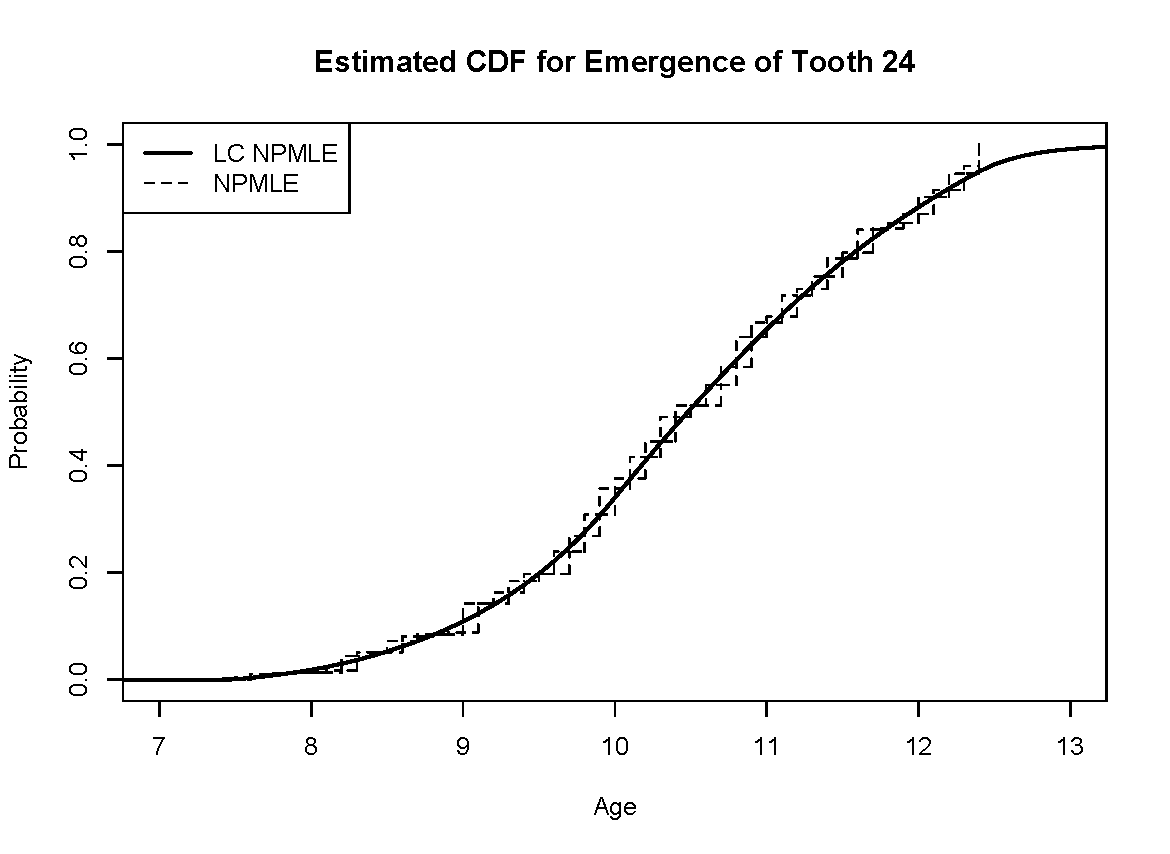
\includegraphics[width = 9cm]{ToothEmergence.pdf}}
\caption{Estimated CDF for Tooth 24 Emergence}
\label{figure:teeth}
\end{figure}		



{\section{Algorithm Speeds}  
\label{sec:AlgSpd}	}

	The complexity of each step of the algorithm is of order $O(u_t u_o)$, where $u_t$ is the number of unique times in the data set and $u_o$ is the number of unique observations (\emph{i.e.} unique pairs of $L_i$ and $R_i$). This dictates that the speed of our algorithm is strongly tied to the number of unique times. In addition, for a given number of unique times, case II interval censored data can be more computationally expensive, as the number of combinations of $L_i, R_i$ is higher than for current status data. 

	To investigate the speed of our algorithm, we computed the log-concave NPMLE across different scenarios. We considered both current status and case II interval censored data across different combinations of sample size and number of unique times. For current status data, both the event time and inspection time were simulated from a gamma(2,2) distribution. For case II interval censored data, the event times were simulated from a beta(2,2) distribution. There were two inspection times, $C_1$ and $C_2$ with $C_1 \sim $ uniform(0, 2/3) and $C_2 \sim$ uniform($C_1$, 1). This resulted in approximately 30\% left censored, 30\% right censored and 40\% interval censored data. Unique times were created by binning the censoring times. 
	
	 %in which both the event time and inspection time was simulated from gamma(2,2) distribution. Binning was used to create the number of unique times. 
	
	\begin{table}
\begin{center}	
\caption[Average Computation Times for our Algorithm]{Average computation times in seconds for our algorithm. ``-" implies combination of $n$ and $u_t$ is invalid (i.e. $u_t > n$) }
\label{table:compTime}
\begin{tabular} {| c | c | c | c | c | c | c | c |} 


	 \hline

		 & \multicolumn{7} {|c|} {Unique Times} \\

		
	\hline	
		
	$n$ & 10 & 50 & 100 & 500 & 1000 & 2000 & 5000\\	

	\hline
		  \multicolumn{8} {|c|} {Current Status Data} \\
		
	 \hline 
 
 	100 & 0.01 & 0.03 & 0.07 & - & - &  - & -\\ 
	
	\hline
	
	500 & 0.01 & 0.04 & 0.10 & 1.38 & - & - & -\\
	
	\hline
	
	5000 & 0.05 & 0.11 & 0.19 & 1.94 & 7.17 & 32.6 & 196 \\ 
	
	\hline
	
	 \multicolumn{8} {|c|} {Case II Interval Censored Data} \\
	 \hline 
 
 	100 & 0.01 & 0.03 & 0.05 & - & - &  - & -\\ 
	
	\hline
	
	500 & 0.02 & 0.08 & 0.14 & 0.91 & - & - & -\\
	
	\hline
	
	5000 & 0.08 & 0.44 & 1.12 & 4.13 & 9.78 & 28.1 & 118 \\ 

	
	\hline
	
\end{tabular}
\end{center}

\end{table}

	In table \ref{table:compTime}, we present average computation time in seconds across different sample sizes and different numbers of unique times in the data using simulated current status data and case II interval censored data. We compared this to the R package logconcens. This was complicated by the fact  that the algorithm in logconcens occasionally failed to converge and (less frequently) failure of the algorithm for other reasons: the two problems observed were reports of inability to invert a Hessian matrix and selection of an undefined index. In order to represent what we considered the most fair comparison, we set the maximum iterations to 1,000 and reported both the average times (even if the algorithm did not converge or failed) and the proportion of times the algorithm did not converge. We looked at sample sizes $n$ = 25, 50 and 100. This can be seen on Table \ref{table:LogConSpd}. 
	
	Examining the tables, we see that our algorithm performs much better than the algorithm in logconcens for interval censored data with regards to speed. In addition, we found that our algorithm resulted in a higher final log likelihood 72\% of the time. The $99^{th}$ and $1^{st}$ percentile of the difference between final log likelihood of our algorithm compared and logconcens's was 0.093 to -0.012, although the large differences may be due to discretization used in logconcens rather than early stopping. It is worth noting that both algorithms use identical stopping criterion. 
\\
	{\begin{table}	
	
\begin{center}	
\begin{tabular} {| c | c | c | c |} 


	 \hline

		 & \multicolumn{3} {|c|} {Unique Times} \\

	\hline
	
		  \multicolumn{4} {|c|} {Current Status Data} \\
		
	\hline	
		
	$n$ & 10 & 25 & 50 \\
		
	 \hline 
 
 	25 &    4.99 (0.17)	& 7.80 (0.05)	& -	\\ 
	
	\hline

 	50 &  6.31 (0.09) 	& 13.6 (0.05)	& 19.7 (0.17)  \\ 
	
	\hline
	
 	100 &  7.66 (0.07)  	& 21.6 (0.05)	&  36.5 (0.16)	   \\ 

	\hline
	
		  \multicolumn{4} {|c|} {Case II Interval Censored Data} \\
		
		
	 \hline 
 
 	25 &   1.61 (0.01) & 5.07(.03)	& -	\\ 
	
	\hline

 	50 &  3.19 (0.01) & 6.65 (0.02)	& 12.1 (0.03)  \\ 
	
	\hline
	
 	100 &  2.54 (0.00)  	& 11.3 (0.00)	&  21.5 (0.03)	   \\ 
	

	
	\hline
	
\end{tabular}
\end{center}

\caption[Average Computation Times for Logconcens Algorithm]{Average computation times in seconds for logconcens. Values in parentheses are proportion of datasets that failed to converge after 1,000 iterations}
\label{table:LogConSpd}
\end{table}
}



	{\section{Empirical Rates of Convergence} 
	\label{sec:Conv}	}
	The unconstrained NPMLE has been shown to have theoretic cube root convergence. Although we do not attempt to derive the theoretic limiting distribution of the log concave NPMLE in this work, we used our algorithm to inspect the empirical rate of convergence via Monte Carlo simulation. In particular, we assume that
	
	\[ ( \hat F (t_0) - F(t_0) ) n^{\beta_1} \rightarrow U_1 \]
	
	and
	
	\[ (\hat F^{-1}(p_0) - F^{-1}(p_0) ) n^{\beta_2} \rightarrow U_2 \]
		
	where $U_1$ and $U_2$ are fixed distributions. Under this assumption, we note that 
	
	\[ \sigma_i (n) \approx c_i \times n^{-\beta_i} \text{ and}	\]
		
	\[ \log( \sigma_i (n) ) \approx \log(c_i) - \beta_i \log(n) \text{, \emph{i} = 1,2} \]	
		
	where $\sigma_i(n)$ is the standard deviation of either $\hat F(t_0)$ or $\hat F^{-1}(p_0)$. 	
	
	To estimate $\beta_1$ and $\beta_2$, we estimated $\sigma_i(n)$ across a range of values for $n$ via simulation and used linear regression on the log transformed values. We used sample size $n = 100$, 200, 400, 800, 1,600, 3,200, 6,400 and 12,800. At each sample size, we used 1,000 simulations to estimate $\sigma(n)$.  We did this both for the log concave NPMLE and the unconstrained NPMLE. Computation of the unconstrained NPMLE was carried out by the R package MLEcens \cite{R_MLEcens}. We considered two different scenarios for the event time: $T_i \sim $ uniform(0,1) and beta (5,5). This was to illustrate our findings that the rate of convergence differed depending on whether the event time distribution was on the boundary of log-concave distributions (\emph{i.e.} uniform(0,1)) or not on the boundary (\emph{i.e.} beta(5,5) ). We considered both a current status scenario and a case II interval censored scenario. We inspected the convergence rate of $\hat F(t_0 = q_{0.50})$ ($q_\alpha$ = $\alpha$ quantile of the true event time) and $\hat Q( p_0 = 0.5)$ ($\hat Q$ is the estimated quantile function), although we also include the estimated standard deviations and biases for $\hat F(t_0 = q_{0.50} )$, $\hat F(t_0 = q_{0.75} )$, $\hat F(t_0 = q_{0.90} )$, $\hat Q(p_0 =0.5 )$, $\hat Q(p_0 =0.75 )$ and $\hat Q(p_0 =0.9 )$ on a subset of the scenarios considered, which are shown on tables \ref{table:SD_Bias_Case_I} and \ref{table:SD_Bias_Case_II}. 

	
	In the current status scenario, we simulated the inspection process according to a  $C \sim $ uniform(0,1).  For the case II interval censored scenario, we considered two inspection times $C_1 \sim$ unif(0,1) and $C_2 \sim$ unif($C_1, 1)$. 
		
	From table \ref{table:EstConRates}, we see the estimated rates of convergence for both the log concave NPMLE (LC NPMLE) and unconstrained NPMLE (UC NPMLE). In all cases, the empirical rate of convergence for the log concave NPMLE was significantly faster than the  unconstrained NPMLE. For the unconstrained NPMLE, we see that the empirical rate of convergence is fairly close to the theoretical rate of 1/3 for current status data. For case II interval censored data, the convergence rate appears faster than the equivalent scenario with current status data in all cases, although the relative improvement is greater for the unconstrained NPMLE than the log concave NPMLE. For the log concave NPMLE, the rate of convergence appeared slightly lower when the event time was well inside the boundary, although still significantly higher than the rate of convergence of the unconstrained NPMLE. This result is consistent with many other exploratory simulations we conducted but did not list in this paper. Our findings suggest that the rate of convergence is dependent on the distance (not properly defined at this time) between the event time distribution and the log concave boundary. 
	
	Examining the estimated standard deviations and biases on tables \ref{table:SD_Bias_Case_I} and \ref{table:SD_Bias_Case_II}, we see that both estimators appear to have a slight downward bias further down on the estimates of the tails. It appears that the bias is less for the log concave estimator, although the bias appears to shrink quickly for both estimators, which is consistent with asymptotic theory that shows that both estimators are consistent. 
	
	Further theoretically derived results would be very helpful for analyzing the advantage gained by using the shape constrained estimator for interval censored data. At this time, we are not aware of any work being done in that area. 
\\


	{\section{Future Work} 
	\label{sec:future}	}
	In the case of the log-concave NPMLE for exact data, uniqueness is shown using the fact that the log likelihood is strictly concave \cite{RefRuf2007}. This cannot be applied to the interval censored case, as the log likelihood function is not always concave. In the case of the univariate unconstrained NPMLE, it has been shown that the solution does not have mixture non-uniqueness (for a solution set of intervals, there is only one assignment of mass to each interval which maximizes the likelihood function) but does suffer from representational non-uniqueness (for a mixed mass and interval, any assignment of mass within the interval leads to the same likelihood \cite{RefGV2001}). The proof depends on the fact that the solution only assigns mass to the Turnbull intervals. In trivial problems, such as a single censored observation, it is clear that the log concave NPMLE can show representational non-uniqueness. However, it is not clear whether the estimator suffers from mixture non-uniqueness. 
	
	Although the algorithm presented in this chapter is acceptable for small to moderate sized data sets or larger data sets with large numbers of ties (see appendix), it would be too slow for larger data sets with large amounts of unique values. For example, in our simulations we found that if $n = 5,000$, all with unique times, the algorithm look over 2 minutes to converge on average (see table 1). In contrast, the CRAN package MLEcens can compute the unconstrained NPMLE for $ n = 5,000$ in 3.85 seconds on average. 
	
	Finally, theoretical results about the limiting distribution and rate of convergence for estimators based on the shape constrained estimator would be very useful for interval censored data. As we noted earlier, consistency for interval censored data has been shown in \cite{RefDea2014}, but at this time we are unaware of any work being done on the limiting distribution of the estimator. This would make comparison of this estimator with competing estimators simpler and provide tools for inference based on the estimator. 
\\			

	{\section{Software}
	\label{sec:software}	}
	
	An implementation of this algorithm can be found on CRAN as a routine in the package logconPH \cite{R_logconPH}. In particular, if the user calls the function \texttt{logconcave} and leaves the argument \texttt{covars} blank, the algorithm presented in this paper will be run. The function also contains a logical argument \texttt{aug}, which will be ignored if the argument \texttt{covars} is blank. Estimated densities, cumulative probabilities and quantiles can be extracted from the fitted object by the functions \texttt{dLC}, \texttt{pLC} and \texttt{qLC} respectively. 
	
	
	In the ICM step, the quadratic program was solved by an implementation of QuadProg++ \cite{QP}, slightly modified to work with R's API. 

	\vspace{1.5cm}

	We would like to thank the anonymous reviewers for helpful advice,  Emmanuel Lesaffre and Dominque Declerck for granting permission for use of the Signal Tandmobiel{\textregistered} Project dataset and George Bergman for help with last minute proofreading.
	
\begin{table}
	
		
\begin{center}

\begin{scriptsize}	

\caption[Test]{Estimated Rates of Convergence, values in parenthesis = 95\% CI}
\label{table:EstConRates}

\vspace{1mm} 
\begin{tabular} {| c | c | c |} 


	\hline	
		
	Scenario							& 	LC NPMLE 		& 	UC NPMLE  \\

	\hline

	&	\multicolumn{2}{| c |}{ Current Status Data }	\\

	\hline	
	
$\hat F(0.5), T\sim U(0,1)$	&	-0.48 (-0.49, -0.47)	&	-0.32 (-0.33, -0.31)	 \\


$\hat F^{-1}(0.5), T\sim U(0,1)$	&	-0.51 (-0.51, -0.50)	&	-0.34 (-0.36, -0.33) \\
	
	\hline
	
$\hat F(0.5), T\sim \beta(5,5)$		&	-0.43 (-0.44, -0.42)	&	-0.31 (-0.33, -0.30)	 \\


$\hat F^{-1}(0.5), T\sim \beta(5,5)$	&	-0.43 (-0.44, -0.42)	&	-0.34 (-0.36, -0.33) \\
	
	\hline	


	&	\multicolumn{2}{| c |}{ Case II Interval Censored Data }	\\

	\hline	


$\hat F(0.5), T\sim U(0,1)$	&	-0.51 (-0.53, -0.50)	&	-0.37 (-0.39, -0.36)	 \\


$\hat F^{-1}(0.5), T\sim U(0,1)$	 	&	-0.50 (-0.52, -0.48)	&	-0.42 (-0.45, -0.38)\\
	
	\hline
	
$\hat F(0.5), T\sim \beta(5,5)$	 &	-0.44 (-0.46, -0.43)	&	-0.36 (-0.38, -0.35) \\


$\hat F^{-1}(0.5), T\sim \beta(5,5)$  	&	-0.45 (-0.46, -0.43)	&	-0.37 (-0.39, -0.34)	\\
	
	\hline	


\end{tabular}
\end{scriptsize}
\end{center}


\end{table}
	



%\begin{acknowledgements}
%If you'd like to thank anyone, place your comments here
%and remove the percent signs.
%\end{acknowledgements}

% BibTeX users please use one of
%\bibliographystyle{spbasic}      % basic style, author-year citations
%\bibliographystyle{spmpsci}      % mathematics and physical sciences
%\bibliographystyle{spphys}       % APS-like style for physics
%\bibliography{}   % name your BibTeX data base

% Non-BibTeX users please use
\begin{thebibliography}{}
%
% and use \bibitem to create references. Consult the Instructions
% for authors for reference list style.
%

\bibitem{R_logconPH}
Anderson-Bergman, C., (2014), logconPH: CoxPH Model with Log Concave Baseline Distribution, http://CRAN.R-project.org/package=logconPH

\bibitem{myThesis}
Anderson-Bergman, C.,  Semi- and Non-parametric Methods for Interval Censored Data with Shape Constraints, Ph.D. Thesis, University of California Irvine, (2014)

\bibitem{RefBB2005}
Bagnoli, M., Bergstorm, T., Log-concave Probability and its Applications, \emph{Economic Theory} Vol 26 No. 2, 445-469, (2005)

\bibitem{R_ICE}
Braun, J., (2013) ICE: Iterated Conditional Expectation, http://CRAN.R-project.org/package=ICE

\bibitem{RefBea2005}
Braun, J., Duchense, T., Stafford, J., Local Likelihood Density Estimation for Interval Censored Data, \emph{The Canadian Journal of Statistics}, Vol 33 No.1, 39-60, (2005)

\bibitem{RefBogLes2004}
Bogaerts, K., and Lesaffre, E., A New, Fast Algorithm to Find the Regions of Possible Support for Bivariate Interval-Censored Data, \emph{Journal of Computational and Graphical Statistics}, Vol 13, No 2, (2004)

\bibitem{RefDFJ2006}
D\"umbgen, L., Freitag-Wolf, S. and Jongbloed, G., Estimating a Unimodal Distribution From Interval-Censored Data, \emph{Journal of the American Statistical Association}, Vol 101 No. 475, (2006)

\bibitem{RefDea2007}
D\"umbgen, L., H\"usler, A., Rufibach, K., Active Set and EM Algorithms for Log-Concave Densities Based on Complete and Censored Data, \emph{preprint}, (2007)

\bibitem{RefDea2014}
D\"umbgen, L., H\"usler, A., Rufibach, K., Maximum Likelihood Estimation of a Log-Concave Density Based on Censored Data, \emph{Electronic Journal of Statistics}, Vol 8, No. 1 1405-1437, (2014)

\bibitem{RefDR2009}
D\"umbgen, L., Rufibach, K., Maximum Likelihood Estimation of a Log-Concave Density and its Distribution Function: Basic Properties and Uniform Consistency, \emph{Bernoulli}, Vol 15 No. 1 40-68, (2009)

\bibitem{RefF1972}
Fedorov, V., \emph{Theory of Optimal Experiments}, Academic Press, (1972) 

\bibitem{QP}
Gaspero, L. (2010), QuadProg++,  http://www.diegm.uniud.it/digaspero/index.php/software/

\bibitem{RefGV2001}
Gentleman, R., and Vandal, A., Computational Algorithms for Censored-Data Problems Using Intersection Graphs, \emph{Journal of Computational and Graphical Statistics}, Vol 10 No. 3, 403-421, (2001)


\bibitem{RefGV2002}
Gentleman, R., and Vandal, A., Nonparametric Estimation of the Bivariate CDF for Arbitrarily Censored Data, \emph{The Canadian Journal of Statistics}, Vol 30 No. 4, 556-571, (2002)

\bibitem{RefGCOL2009}
Gomez, G., Calle, M., Oller, R., and Langohr, K., Tutorial on Methods for Interval-Censored Data and Their Implementation in R, \emph{Statistical Modelling}, Vol 9 No. 4 259-297, (2009)

\bibitem{RefG1987}
Groeneboom, P., Asymptotics for Interval Censored Observations, \emph{Technical Report} 87-18. Department of Mathematics, University of Amsterdam, (1987) 

\bibitem{RefG1991}
Groeneboom, P., Nonparametric Maximum Likelihood Estimation for Interval Censored Data, \emph{Technical Report}, Statistics Department, Stanford University, (1991)

%\bibitem{RefStraweib}
%Gu, X., and Balasubramanian, R., straweib: Stratified Weibull Regression Model, http://cran.r-project.org/web/packages/straweib/index.html

\bibitem{RefH1999}
Huang, J., Asymptotic properties of nonparametric estimation based on partly interval-censored data, \emph{Statistica Sinica}, Vol 9, 501-519, (1999)

\bibitem{RefJ2003}
Jewell, N., Laan, M., Henneman, T., Nonparametric Estimation from Current Status Data with Competing Risks, \emph{Biometrika}, Vol 90 No 1, 183-197, (2003)

\bibitem{RefJ1998}
Jongbloed, G., The Iterative Convex Minorant Algorithm for Nonparametric Estimation, \emph{Journal of Computational and Graphical Statistics}, Vol 7, No. 3, 310-321, (1998)


\bibitem{R_BayesSurv}
Kom\'arek, A., (2104) bayesSurv: Bayesian Survival Regression with Flexible Error and Random Effects Distributions, http://cran.r-project.org/web/packages/bayesSurv/index.html


\bibitem{RefKL2006}
Kom\'arek A., and Lesaffre E., Bayesian Semi-Parametric Accelerated Failure Time Model for Paired Double-Interval-Censored Data, \emph{Statistical Modelling} Vol 6 3-22, (2006)

\bibitem{RefKL2009}
Kom\'arek A., and Lesaffre E., The Regression Analysis of Correlated Interval-Censored Data: Illustration using Accelerated Failure Time Models with Flexible Distributional Assumptions, \emph{Statistical Modelling} Vol 9 No. 4 299-319, (2009)


\bibitem{RefKS1992}
Kooperberg, C., and Stone, C., Logspline Density Estimation for Censored Data, \emph{Journal of Computational and Graphical Statistics}, Vol 1, 301-328, (1992)

\bibitem{R_logSpline}
  Kooperberg, C., (2013), logspline: Logspline density estimation routines, http://CRAN.R-project.org/


\bibitem{RefKKT1951}
Kuhn, W., Tucker, W., Nonlinear Programming, \emph{Proceedings of 2nd Berkeley Symposium}, 481-492 (1951)

\bibitem{RefLKD2005}
Lesaffre, D., Kom\'arek, A., and Declerck, D., An Overview of Methods for Interval-Censored Data with an Emphasis on Applications in Dentistry, \emph{Statistical Methods in Medical Research}, Vol 14, 539-552, 2005

\bibitem{R_MLEcens}
Maathuis, M., (2013), MLEcens: Computation of the MLE for bivariate (interval) censored data, http://CRAN.R-project.org/package=MLEcens


\bibitem{RefP2000}
Pan, W., Smooth Estimation of the Survival Function for Interval Censored Data, \emph{Statistics in Medicine}, Vol 19, No. 19, 2611-2624,  (2000)

\bibitem{R}
R Core Team, (2014) R: A Language and Environment for Statistical Computing, http://www.R-project.org/

\bibitem{RefRuf2006}
Rufibich, K., Log-Concave Density Estimation and Bump Hunting for i.i.d. Observations. Ph.D. dissertation, Univ. Bern and G\"ottingen (2006)


\bibitem{RefRuf2007}
Rufibach, K., Computing Maximum Likelihood Estimators of a Concave Density, \emph{Journal of Statistical Computation and Simulation}, Vol 77, No. 7, 561-574, (2007)

\bibitem{R_logconcens}
Schuhmacher, D., Rufibach K., and D\"uembgen, L., (2013), logconcens: Maximum likelihood estimation of a log-concave density based on censored data, http://CRAN.R-project.org/package=logconcens


\bibitem{RefT1976}
Turnbull, B., The Empirical Distribution Function with Arbitrarily Grouped, Censored and Truncated Data, \emph{Journal of the Royal Statistical Society. Series B (Methodological)}, Vol 38, No. 3 290-295 (1976)

\bibitem{RefVan2000}
Vanobbergen J., Lesaffre E. and Declerck D., The Signal-Tandmobiel {\textregistered} Project - a Longitudinal Intervention Health Promotion Study in Flanders (Belgium): Base and First Year Results, \emph{European Journal of Pediatric Dentistry}, Vol 2, 87-96 (2000) 


% etc
\end{thebibliography}




{\section{Appendix}  	
\label{sec:app}	}

	\subsection{Proof of Theorem \ref{thm2}}
	
	We state the following theorem about the likelihood function for the log-concave NPMLE for interval censored data:
		
	The likelihood function is continuous, coercive and bounded (and therefore has a maximum) if there exist $i,j \in 1, ... , n$ such that $L_i > R_j$. To show this, we consider the following three cases.
	
	1. At least two data points are uncensored, and they are not equal to each other
	
	2. All the data are censored
	
	3. There exists one uncensored data point which is not contained in at least one of the censored intervals
		
	\begin{proof}
	
	In all three cases, continuity is trivial; the likelihood function is a sum of continuous functions. 
	
	For case 1, coercivity and boundedness are easily proven given that it has been shown that the log likelihood function for uncensored is strictly concave when at least two unique values are observed \cite{RefRuf2006}. We can consider the log likelihood function as having contributions from the censored and uncensored data. Because the contributions of the censored must be non-positive, the sum of uncensored and censored observations is bounded from above by the contribution of the uncensored observations. Because the contribution of the uncensored observations has been shown to be strictly concave, and the total likelihood is bounded from above by the contribution of the uncensored observations, the total likelihood is bounded and coercive. 
	
	For case 2, we again use the fact that the contribution of the censored observations is bounded from above by 0. Therefore, the log likelihood function is bounded. To show that the likelihood function is coercive, consider if one of the standardized $\beta_k$'s approaches $\infty$. Because the standardized $\beta_i$'s must describe a proper probability distribution, as $\beta_k \rightarrow \infty$, $\beta_l \rightarrow -\infty$ for all $l \neq k$. Thus, the contribution to the likelihood function for any observation interval not containing $\beta_k$ will approach $-\infty$ as $\beta_k \rightarrow \infty$. Since $L_i > R_j$ implies there exists at least one interval such that $\beta_k$ is not within this interval, the contribution of this interval will approach $-\infty$ as $\beta_k \rightarrow \infty$, while all other intervals will be bounded from above by 0. Therefore, the likelihood function is coercive. 
	
	For case 3, first we note that the only complication is when there is only one unique time. If there is more than one unique time, this could be considered case 1 which has already been established. It is worth noting that there can be multiple observations all occurring at the same time, so one could have multiple exact observations without qualifying as case 1. If there are $n_1$ uncensored observations at time $x_1$ and $n_2$ censored observations, the log likelihood function can be written as
	
	\[
	\ell (\phi) = \displaystyle  n_1\phi(x_1) + \sum_{i = n_1+ 1} ^{n_1 + n_2} \log \left( \int_{L_i}^{R_i} e^{\phi(x) } \mathrm{d}x \right)
	\]
	
	Suppose $L$ and $R$ are the end points of an interval such that the unique uncensored time is not within it. Then because the contribution of the other censored observations is less than 0, we have
	
	\[
	\ell(\phi) \leq n_1 \phi(x_1) + \log \left( \displaystyle \int_L^R e^{\phi(x)} \mathrm{d}x \right)
	\]
	
	Noting that the right side of the above equation is bounded below 0. Therefore, if any of the densities approach $\infty$ inside $[L, \infty)$, $\phi(0)$ will approach $-\infty$ (because of the log concave constraint), as will the likelihood function. We must also show that if $\ell(\phi) \rightarrow -\infty$ whenever $\phi(x_1) \rightarrow \infty$. 
	
	Without loss of generality, let us assume that $x_1 = 0$ and $L > 0$. Then we have that 
	
	\[
	 \ell(\phi) \leq n_1 \phi(0) + \log \left( \displaystyle \int_L^R e^{\phi(x)} \mathrm{d}x \right) 
	\]
	
	\[
	\ell(\phi) \leq n_1 \phi(0) + \log \left( \displaystyle \int_L^\infty e^{\phi(x)} \mathrm{d}x \right)
	\]

	We note that for any choice of $\phi(0)$, $\log \left( \displaystyle \int_L^\infty e^{\phi(x)} \mathrm{d}x \right) $ is maximized by setting $\phi(x)$ to be an exponential distribution with rate $\lambda = e^{\phi(0)}$. This can be seen readily from the fact that the exponential distribution is the limit of the log-concave constraint. This means we can use the cdf of the exponential distribution to further bound the likelihood, \emph{i.e.}, setting $\phi(0) = \log(\lambda)$, we get 
	
	\[
	\ell(\phi) \leq n_1 \log(\lambda) + \log( e^{- \lambda L} ) = n_1 \log(\lambda) - \lambda L
	\]
	
	Because $L > 0$, as $\lambda \rightarrow \infty$ the above equation approaches $-\infty$. Therefore, the likelihood function is bounded and coercive. 
	\\
	\end{proof}


\begin{table}
\caption[Test]{Estimated standard deviations and biases for simulated current status data based on 1,000 simulations. Event times $T \sim \text{beta}(5,5)$, inspection times $C \sim \text{unif}(0,1)$.  LC = log concave NPMLE, UC = unconstrained NPMLE. First value is estimated standard deviation of estimate, second value (in parentheses) is estimated bias. * indicates the estimated bias is statistically significant}
\begin{center}
\label{table:SD_Bias_Case_I}
\begin{tabular}{| c | c | c | c |  c | }

\hline
		\multicolumn{2}{|c|}{Estimand} & \multicolumn{3} {|c|} {Current Status Data}   \\
		 
	\hline
	
	
						\multicolumn{2}{|c|}{n}	&	 100			& 400 	& 1600		\\
	
	\hline

	\multirow{4}{*}{$\hat F(q_{0.50})$}	& \multirow{2}{*}{LC}		&	0.096		& 0.052		& 0.028		\\
						&					&	(0.006)		& (0.000)		& (0.000)		\\	
	
						\cline{2- 5}
	
						& \multirow{2}{*}{UC}		&	0.159		& 0.090		& 0.056		\\
						&					&	(0.009)		& (-0.005)		& (-0.001)		\\
	\hline										
	
	\multirow{4}{*}{$\hat F(q_{0.75})$}	& \multirow{2}{*}{LC}		&	0.094		& 0.048		& 0.025		\\
						&					&	(-0.008)		& (0.002)		& (0.000)		\\	
						
						\cline{2- 5}
						
						& \multirow{2}{*}{UC}		&	0.141		& 0.081			& 0.049		\\
						&					&	(-0.017)*		& (-0.010)*		& (0.000)		\\
	\hline

	\multirow{4}{*}{$\hat F(q_{0.90})$}	& \multirow{2}{*}{LC}		&	0.068		& 0.035			& 0.018	\\
						&					&	(-0.018)*		& (-0.004)*		& (0.001)	\\	
	
						\cline{2- 5}
		
						& \multirow{2}{*}{UC}		&	0.090		& 0.055		& 0.032		\\
						&					&	(-0.031)*		& (-0.010)*	& (-0.001)		\\
	
	\hline


	\multirow{4}{*}{$\hat Q(0.5)$}	& \multirow{2}{*}{LC}	&	0.037		& 0.022	& 0.011	\\
						&					&	(-0.002)		& (0.000)	& (0.000)	\\	
	
						\cline{2- 5}
	
						& \multirow{2}{*}{UC}		&	0.057		& 0.038		& 0.022	\\
						&					&	(-0.008)*		& (-0.008)*	& (0.001)	\\
	
	\hline										
	
	\multirow{4}{*}{$\hat Q(0.75)$}	& \multirow{2}{*}{LC}	&	0.039		& 0.023	& 0.012	\\
						&					&	(0.002)		& (-0.001)	& (0.000)	\\	
	
						\cline{2- 5}
	
						& \multirow{2}{*}{UC}		&	0.059		& 0.038	& 0.024	\\
						&					&	(-0.010)*		& (-0.001)	& (0.003)*	\\
	\hline

	\multirow{4}{*}{$\hat Q(0.90)$}	& \multirow{2}{*}{LC}	&	0.052		& 0.026	& 0.015	\\
						&					&	(0.014)*		& (0.003)*	&(0.000)	\\	
	
	
						\cline{2- 5}
	
						& \multirow{2}{*}{UC}		&	0.072		& 0.043	& 0.027	\\
						&					&	(0.031)*		& (0.010)*	& (0.003)*	\\

		

\hline



\hline

%//	$F(0.5)$	
\hline


\end{tabular}
\end{center}
\end{table}



\begin{table}
\caption[Test]{Estimated standard deviations and biases for simulated case II interval censored data based on 1,000 simulations. Event times $T \sim \text{beta}(5,5)$, inspection times $C_1 \sim \text{unif}(0,2/3)$ and $C_2 \sim \text{unif}(C_1, 1)$.
LC = log concave NPMLE, UC = unconstrained NPMLE. First value is estimated standard deviation of estimate, second value (in parentheses) is estimated bias. * indicates the estimated bias is statistically significant}
\begin{center}
\label{table:SD_Bias_Case_II}
\begin{tabular}{| c | c | c | c |  c | c | c | c |}

\hline
		\multicolumn{2}{|c|}{Estimand} &  \multicolumn{3} {|c|} {Case II Interval Censored Data}   \\
		 
	\hline
	
	
						\multicolumn{2}{|c|}{n}	&	 100		& 400 	& 1600	\\
	
	\hline

	\multirow{4}{*}{$\hat F(q_{0.50})$}	& \multirow{2}{*}{LC}			& 0.066		& 0.036	& 0.019	\\
						&						& (0.002)		& (-0.001)	& (-0.001)	\\	
	
						\cline{2- 5}
	
						& \multirow{2}{*}{UC}			& 0.110		& 0.067	& 0.040	\\
						&						& (0.003)		& (-0.001)	& (-0.001)	\\
	\hline										
	
	\multirow{4}{*}{$\hat F(q_{0.75})$}	& \multirow{2}{*}{LC}			&0.062		& 0.031	& 0.017	\\
						&				 		& (0.000)		& (0.001)	& (-0.001)	\\	
						
						\cline{2- 5}
						
						& \multirow{2}{*}{UC}			& 0.100		& 0.054	& 0.031	\\
						&						& (-0.005)		& (-0.001)	& (-0.001)	\\
	\hline

	\multirow{4}{*}{$\hat F(q_{0.90})$}	& \multirow{2}{*}{LC}			& 0.052			& 0.025	& 0.014	\\
						&						& (-0.009)*		& (0.001)	& (0.000)	\\	
	
						\cline{2- 5}
		
						& \multirow{2}{*}{UC}			& 0.075			& 0.043	& 0.026	\\
						&						& (-0.016)*		& (0.001)	& (0.000)	\\
	
	\hline


	\multirow{4}{*}{$\hat Q(0.5)$}	& \multirow{2}{*}{LC}		& 0.027		& 0.015	& 0.008	\\
						&						& (-0.001)		& (0.001)	& (0.000)	\\	
	
						\cline{2- 5}
	
						& \multirow{2}{*}{UC}			& 0.044		& 0.028	& 0.016	\\
						&						& (0.000)		& (0.001)	& (0.001)	\\
	
	\hline										
	
	\multirow{4}{*}{$\hat Q(0.75)$}	& \multirow{2}{*}{LC}		& 0.029		& 0.016	& 0.008	\\
						&						& (0.000)		& (-0.001)	& (0.000)	\\	
	
						\cline{2- 5}
	
						& \multirow{2}{*}{UC}			& 0.044		& 0.026	& 0.016	\\
						&						& (0.003)		& (0.002)	& (0.001)	\\
	\hline

	\multirow{4}{*}{$\hat Q(0.90)$}	& \multirow{2}{*}{LC}		& 0.037		& 0.019	& 0.011	\\
						&						& (0.006)*		& (-0.001)	& (0.000)	\\	
	
	
						\cline{2- 5}
	
						& \multirow{2}{*}{UC}		& 0.054		& 0.033	& 0.021	\\
						&					& (0.017)*		& (0.001)	& (0.002)*	\\

		

\hline



\hline

%//	$F(0.5)$	
\hline


\end{tabular}
\end{center}
\end{table}



\end{document}
% end of file template.tex

